\section{LOV and OSC}

From a high level perspective, the job of LOV is to direct pages to the correct
OSCs and OSC's job is to assemble a vector of dirty pages, group them, and send them
to OST over the wire (of course, through the Portal RPC and LNET).


\subsection{OBD Device Operations}

One of the general code organization patterns or implementation techniques employed
and that can be seen across LOV, OSC, and MDC are \textit{obd device oriented
operations}. An obd device is characterized by a method table defined by
\url{struct obd_ops}, somewhat similar to the aforementioned VFS file, inode,
dentry operations. The idea is that you can be insulated from knowing the exact
obd devices you are talking to and use the generic wrapper method prefixed by
\url{OBD_} instead.  Let's take a glimpse of the methods this table defines:

\begin{Verbatim}
struct obd_ops {
    struct module * o_owner;
    int (o_setup)(struct obd_device *dev, obd_count len, void *data);
    int (o_attach)(struct obd_device *dev, obd_count len, void *data);
    int (o_detach)(struct obd_device *dev);
    int (o_setattr)(struct obd_export *exp, struct obd_info *oinfo ...);
    ...
}
\end{Verbatim}

Although there are over 70 methods defined in the structure, only a small set
of methods are supported across the board. Therefore, it has lost the
generic character that was originally envisioned. Nonetheless, this method
table provides a roadmap for us to explore activities around the particular obd
devices.

For LOV, another pattern to note is that this is the layer that interprets
stripe information; therefore, a file operation here often becomes an
operation on a set of objects. 

When LOV module initializes, it registers the obd device operations it
supports to a class type manager. Essentially, this class type manager
manages a class name and its associated properties in a flat space.

\begin{Verbatim}
rc = class_register_type(&lov_obd_ops, lvars.module_vars, LUSTRE_LOV_NAME);
\end{Verbatim}

\subsection{Page Management}

Page management is an activity across multiple layers.  Page cache is a
generic memory space maintained by the kernel.  Lustre pages are just those
special pages the Lustre system is aware of. The special properties are stored in
the private field of a page descriptor.  It is divided into three portions:
\url{llap}, \url{lap} and \url{oap}. The responsible layer that will do
manipulation on its portion are \url{llite}, \url{lov} and \url{osc},
correspondingly, as illustrated below:

\begin{Verbatim}   
<-- llite --> <-- lov --> <-- osc  --> 
+------------+-----------+-----------+
|    llap    |    lap    |    oap    |
+------------+-----------+-----------+
\end{Verbatim}

To keep this discussion more tangible, we will refer to the following use case
from time to time to keep us focused: A user space application wants to create
file $A$, then write 6.5MB of data to it. The stripe size is 1MB, stripe width
is 3, and OSTs are numbered as $OST_1$, $OST_2$, and $OST_3$. The file A's data
objects are named $A_1$, $A_2$, and $A_3$, correspondingly.  The other files
on these particular OSTs will be called $B_1$, $B_2$, $B_3$ and $C_1$, $C_2$,
$C_3$, as illustrated in Figure~\ref{fig:lite_example}.  At this point, we need
to define or clarify a few concepts and data structures.  At VFS and Lustre
Lite layers, the read and write happens on the page unit -- note that it has no
bearing on the actual data transfer done by Portal RPC and LNET. 
 
\begin{figure}[hbt]
\centering
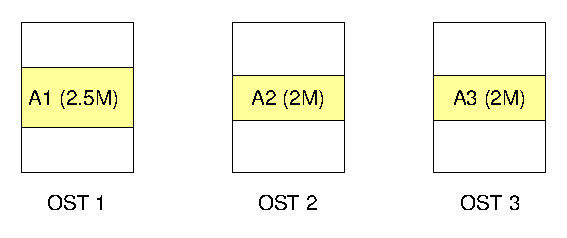
\includegraphics[width=3in]{img/lite_example}
\caption{Lustre Lite object placement example.}
\label{fig:lite_example}
\end{figure}

 
A page of data needs to find its home on a file data object on
the OST disk. The location information is essentially a tuple of
     $<$\textit{OST index},
     \textit{offset within file data object in page unit},
     \textit{offset within page}$>$.
Here is how it is defined:

\begin{Verbatim}
struct lov_async_page {
    int         lap_stripe;     /* same as OST logical index */
    obd_id      lap_loi_id;     /* object id as seen by OST */
    obd_off     lap_sub_offset; /* offset within object in page-unit */
    ...
}
struct osc_async_page {
    obd_off     oap_obj_off;    /* offset within object in page unit */
    unsigned    oap_page_off;   /* offset within a page */
    ...
}
\end{Verbatim}

\subsection{From OSC Client To OST}

To interact with an OST, the client side needs to create a corresponding OSC client
structure, \url{client_obd}. This is a one-to-one mapping.  Note that
\url{client_obd} represents other clients such as MGC, MDC as well. So in that
sense, it is fairly generic and some fields may only make sense for a
particular client.

For each data object handled by OSC client, there is one \url{lov_oinfo}
object (loi) created, and each describes an object associated the OST. Each
\url{lov_oinfo} further links to OAP pages for both read and write.

The \url{lov_oinfo} struct has a link back to \url{client_odb}, therefore, it
can be used as the starting point, to search all \url{lov_oinfo} for each
object this client is processing and to continue to locate all OAP pages
that have been cached dirty during the write operation.

\begin{figure}[htb]
\centering
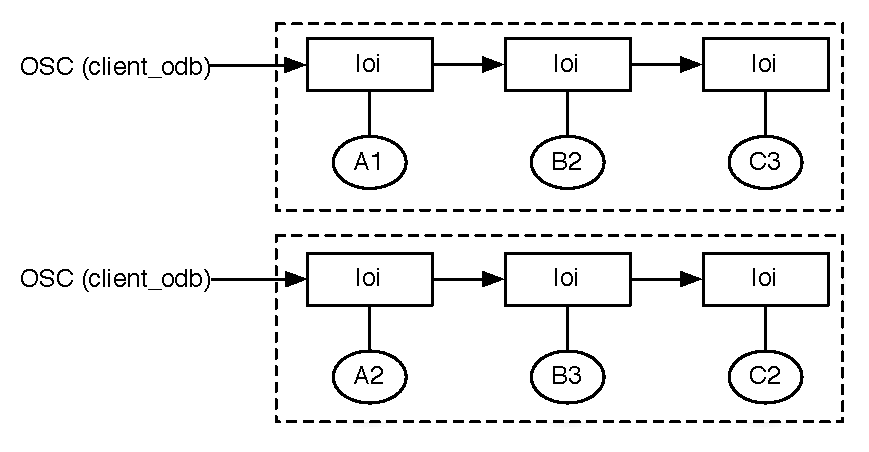
\includegraphics[width=3.5in]{img/client_loi}
\caption{Connecting OSC client, \texttt{lov\_oinfo} and OST objects.}
\label{fig:client_loi}
\end{figure}

Figure \ref{fig:client_loi} illustrates the case where two OSC clients interact
with two OSTs.  The first OST holds data objects of $A_1$, $B_2$, and $C_3$;
the second OST holds $A_2$, $B_1$.

\subsection{Grant}

Each client buffers some amount of dirty data. Currently, the default setting
for each OSC is 32 MB.\footnote{This is tunable through proc filesystem.}
Considering the number of clients we can have in the system, it is easy to see
that when all clients flush their dirty buffer, the server side
might run out of free space on the filesystem.  To avoid this situation,
the server establishes a certain limit on the amount of dirty data it can
flush or transfer for each client, known as the \textit{grant}. Clients are not
allowed to have more dirty data than the grant. Clients can ask for more, and the
server exercises the discretion to increase the grant and by how much.  It is adjusted
according to the amount of dirty data the client is caching. Every time a client
dirties a page, it is subtracted from that grant. When grant reaches zero, all I/O
becomes synchronous until the client can increase its grant.
